%-----------------------------------------------------
% index key words
%-----------------------------------------------------
\index{vector}
\index{vector arithmetic}

%-----------------------------------------------------
% name, leave blank
% title, if the exercise has a name i.e. Hilbert's matrix
% difficulty = n, where n is the number of stars
% origin = "\cite{ref}"
%-----------------------------------------------------
\begin{Exercise}[
name={},
title={}, 
difficulty=0,
origin={\cite{GHC}}]
Sketch $\vec u$, $\vec v$, $\vec u+\vec v$ and $\vec u-\vec v$ on the same axes.
\begin{multicols}{2}
\Question 
\begin{minipage}[m]{\linewidth}
\centering
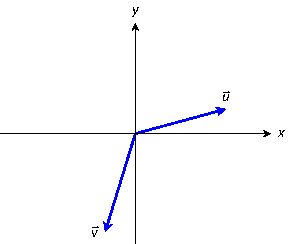
\includegraphics[width=\linewidth]{vector_geometry/introduction_to_vectors/figures/fig10_02_ex_11}
\end{minipage}
\Question
\begin{minipage}[m]{\linewidth}
\centering
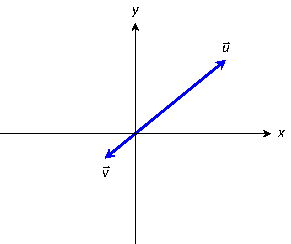
\includegraphics[width=\linewidth]{vector_geometry/introduction_to_vectors/figures/fig10_02_ex_13}
\end{minipage}
\Question
\begin{minipage}[m]{\linewidth}
\centering
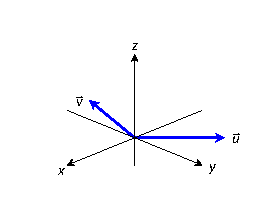
\includegraphics[width=\linewidth]{vector_geometry/introduction_to_vectors/figures/fig10_02_ex_14}
\end{minipage}
\Question
\begin{minipage}[m]{\linewidth}
\centering
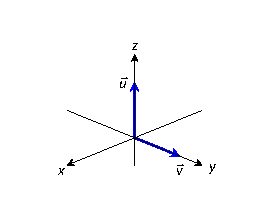
\includegraphics[width=\linewidth]{vector_geometry/introduction_to_vectors/figures/fig10_02_ex_15}
\end{minipage}
\EndCurrentQuestion
\end{multicols}
\end{Exercise}
\begin{Answer}
\Question
\begin{minipage}[m]{\linewidth}
\centering
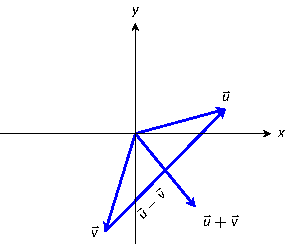
\includegraphics[width=\linewidth/2]{vector_geometry/introduction_to_vectors/figures/fig10_02_ex_11ans}
\end{minipage}
\Question
\begin{minipage}[m]{\linewidth}
\centering
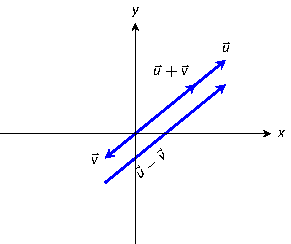
\includegraphics[width=\linewidth/2]{vector_geometry/introduction_to_vectors/figures/fig10_02_ex_13ans}
\end{minipage}
\Question
\begin{minipage}[m]{\linewidth}
\centering
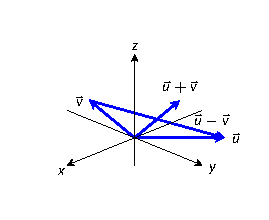
\includegraphics[width=\linewidth/2]{vector_geometry/introduction_to_vectors/figures/fig10_02_ex_14ans}
\end{minipage}
\Question
\begin{minipage}[m]{\linewidth}
\centering
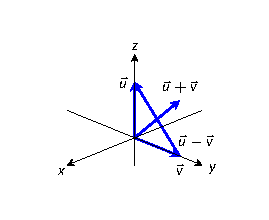
\includegraphics[width=\linewidth/2]{vector_geometry/introduction_to_vectors/figures/fig10_02_ex_15ans}
\end{minipage}
\end{Answer}
